\chapter{Method}\label{cha:Method}

% längsta avsnittet i rapporten. Den består av en redogörelse av ditt arbete och den visar hur du kommer fram till dina resultat.

% Undvik egna synpunkter. Dessa framförs i Inledningskapitlet och Diskussions-kapitlet

% Ange källa till figurer i slutet. T.ex.  Source: Expedition Mondial.

% Metoddelen beskriver tillvägagångssättet – intervjuer, observationer, litteraturstudier, laborationer och så vidare. Motivera varför en viss metod valdes och vilka eventuella svårigheter som har förekommit. Metoden ska vara replikerbar, vilket innebär att en annan skribent ska kunna göra om studien med hjälp av informationen i metoddelen. Det finns en mängd böcker om olika vetenskapliga metoder. Till exempel kan en intervju utföras på en mängd olika sätt. I rapporter inom humaniora brukar metoddelen vara mer utförlig än i en teknisk rapport.

Using novel methods like \textit{service design} when developing the app according to research question \#1 and \textit{data-driven design} and interviews for understanding interaction according to research question \#2.

\section{Preparations in Sweden}

These were the insights before going to Uganda, addressed in the initial work plan.

\section{Answering research questions \#1}

\textbf{\textit{How the topic of Entrepreneurship affects the work}}\\
The scope of the app is to examine the entrepreneurship the student already has. The goal is to give good feedback.

Entrepreneurship is a developing area of research. The topic and the YoungDrive's methology largely effects the work, via its ethos "Dream big, start small", "Can you sell?", and emphasis on fun. Their existing training material and the structure of the program needs to be taken in consideration.

Entrepreneurship means using a learning by doing methodology. A challenging part of the work is that YoungDrive consists of both the practical skills of the entrepreneur, theoretical material of running a business, and an entrepreneurial mindset. Therefore, both how to assess knowledge, and build habits, needs to be examined.

\textbf{\textit{How a Physical education affects the work}}\\
The physical vs. digital interplay needs to be closely examined. How does the app interplay with the physical education? For this, service design methodology will be used. \\

\textbf{\textit{How the Time Constraints and Cultural Differences affects the work}}\\

The biggest challenge with regards to time constraints and cultural differences is that it is difficult to understand the audience.\\

Action:
\begin{itemize}
    \item It led to me started planning the master thesis several months ago
    \item It led to me choosing to spend 3 months in Uganda, because the client and academy is there, and start the design process when I'm there
    \item It led me to the topic of Service Design
\end{itemize}

Positives:
\begin{itemize}
    \item I will come closer to the client and coaches by moving to Uganda, which is necessary when taking a service design approach
\end{itemize}

Negatives:
\begin{itemize}
    \item I will have limited internet outside of the work location
    \item Long distances between work place and home compared to Sweden
    \item I will still have long distances and limited access to coaches\\
\end{itemize}

These negatives needs to be overcome, by narrowing down the scope of the thesis work. \\

\textbf{\textit{How the Design Constraints affects the design process}}\\
"Simple" in this cultural setting leads to design constraints and that design methodology becomes very important.\\

\textbf{\textit{How the Technical Constraints affects the technologies used}}\\
Limitations on internet/electricity means:

\begin{itemize}
    \item Web app
    \item Localized
    \item Database
    \item Fetch/pull functionality in the app
    \item Battery preserving app needed
\end{itemize}

Also, me as a developer have limited experience of building apps, and time constraints. As such, technical compromises should be made.

Furthermore, existing tools could be used, instead of building the app from scratch. E.g. using existing tools like Knowly or Typeform\footnote{examples include https://showroom.typeform.com/to/ggBJPd and https://showroom.typeform.com/report/njdbt5/dIzi} during the first iterations for understanding users, and during development e.g. the Typeform API (http://typeform.io/). The Typeform API allows developers to create surveys from within their own applications or systems. \\


\subsection{Considerations, answering research question \#2}

\subsubsection{Consequences}

To be able to answer research question \#2, evaluation needs to be done. \textbf{\textit{How the Evaluation affects the development process: }} If no evaluation, there would be no need to write code, instead of working with a hi-fi prototype by using existing design tools. Now, we want to use a data-driven approach to measure, and therefore an app needs to be developed.\\

\subsubsection{How to measure}

Answering research question \#2 is a matter of choosing how to measure effectiveness. After choosing what should be evaluated, there needs to be a careful balance between what should be understood via interviews with the target group, and data collection via the app. There are three main aspects that are interesting:

These ways of measuring the questions are subject to change.

%Effectiveness measurements.

\begin{itemize}
    \item 
    \textbf{How do users interact with the app?} (Usability) Give the users a mandatory task (e.g. use the app once a week), and see if they use it more on a voluntary basis, in order to determine if they use the app 
    \textit{(Measure)} and determine why \textit{(Interview and Measurement)}. "Have you during the latest week felt that you've needed any support? Have you then used the app? Did the app help? Or have you searched for support elsewhere?" 
\item \textbf{What usability aspects are associated with using the app?} (Usability) Do they like it? Ask: Are they stimulated? If not, why? What didn't they like? \textit{(Interview)} When can they use the app, and when are they not able to?
    
    \item \textbf{What learning outcomes are associated with using the app for the coaches?}  (Learning of Entrepreneurial Knowledge))
    How good are they at answering the questions? 1. 
    \textit{(Measure)} What percentage of the answers were correct/inorrect?  2. \textit{(Interview)} Were the answers were correct/incorrect because of lack of knowledge or wrong formulated?
    
    Ask the teacher/country manager/project leader if they got valuable information. Ask: did it help them become a better teacher? Were the results trustworthy? \textit{(Interview)}
    
    Do they want to improve their knowledge via the app? This can be measured via how many times they repeat a test, what material they are studying for (e.g. measuring active time spent reading each section).
\end{itemize}

\section{Chosen Design and Development Process}
%Har gått igenom planeringsrapporten lite noggrannare idag och ser två saker som vi kanske ska borde fånga upp under arbetets gång.

% Under 2 Purpose står det ett upplevelsemål från Young Drive. Bör vi mäta detta upplevelsemål om det stämmer med deltagarnas faktiska upplevelse, d v s ska vi försöka få in det under 3 Research Questions?

% På våra avstämningsmöten borde vi också följa upp dina Research Questions så att kundinteraktionerna och servicedesignmetoden tyligt leder dig framåt mot dessa mål.
%* Reflektioner på vilka designprinciper som bör väljas? (utifrån kundinteraktioner)
%* Reflektioner angående tekniska begränsningar?
%* Reflektioner på processen?

I'm the computer expert kind of designer, but aspiring to be a socio-technical expert (which e.g. Expedition Modial are, as service design experts).

Expedition Mondial will help with a method for creating a MVP of the digital support for the coaches, so that the app is developed from the perspective of the end users and the education and a "learning by doing" mentality. The suggested design process was designed with them after a start-up meeting on Skype, and an Education day in Stockholm. During that day a crash course in service design was given, then creating a common plan for the future work based on my needs.

The result is that the design and development phase in Uganda is an iterative process with the human in focus. The process is built on top of service design process and methodology. There are three iterations.

Expedition Mondial will give support in each iteration, helping with the design of each iteration, and the are able to educate me and assists with the different stages and methodologies. They will assist with recommendations on service design literature, and can highlight reports, previous studies, etc.

Each Interactions phase consists of meeting with two coach groups (one with the app and one without the app), to be able to compare the two and measure effectiveness for research question \#2.

Lena Tibell's and Konrad Schönborn's  competence is extremely valuable to me when formulating questionnaires. How to frame the questions is an art.  Therefore in preparation for meetings with the target group we should discuss exactly what I want to know and they will help to phrase the questions. Then, Expedition Mondial can examine the questions from their a development setting.

The trigger material is used in the Interactions phase of the new iteration. This process you can loop as many times as possible, but the Master Thesis is divided into three iterations.

\begin{figure}[h]
    \centering
    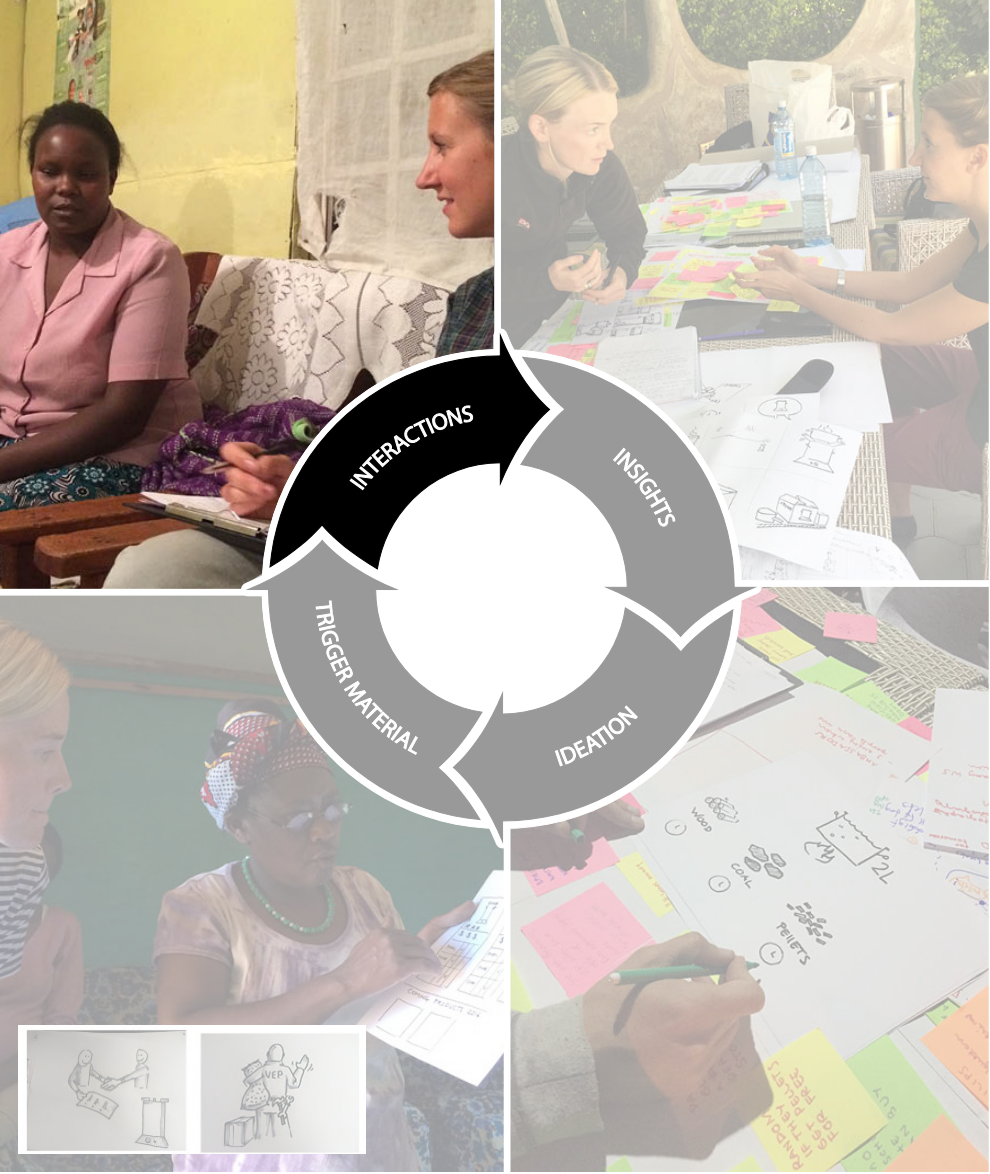
\includegraphics[width=0.7\textwidth]{Iteration.png}
    \caption{One iteration consists of Interactions, Insights, Ideation and Trigger material. The \textbf{Didactic phase} in this figure involves Insights, Ideation and Trigger material. By learning what works and not, new ideas emerge and app design is made, as well as questionnaires for evaluation. The \textbf{Technical phase} in this figure involves to code the improved app design, and evaluate how it works technically.}
    \label{fig:iteration}
\end{figure}

Each iteration ends with two check-up meetings. The first meeting is with the Experts. The next meeting is with the Partners.

The Expert group consists of Expedition Mondial and LiU Innovation. In Expert meetings, I share with them my needs. Expedition Mondial can help with the design process, and LiU Innovation can help if additional resources are needed. The meeting lasts for one hour.

The Partner group consists of most notably Iliana Björling, and preferably also Lena Tibell and Konrad Schönborn. In Partner meetings, The Analysis for the iteration is presented and discussed. Then I will propose possible decisions and discuss the alternatives. % Then I tell them about which decisions has been taken and why.
Finally, we conclude if the master thesis work is going in the right direction. These meetings should be causual and friendly, and not take a lot of time to prepare, so the next iteration can be of focus. % "Kan vara ganska vänskapligt, håll det så enkelt som möjligt så jag får tid till annat."

The time plan for the design and development phase can be seen in the section "In Uganda". The three iterations is presented below: \\

\textbf{The iterations} \\
This is how I want the process to continue:\\

	\textit{\textbf{Iteration 1}}\\
    The first iteration will have a very broad scope. The focus is on the coaches' needs, motivations, and context.  After creation of questions for questionnaire 1, I'll do interviews with coaches and other involved parties. If coaches are met in-group, open questions and dialogue will be done in group for them to be comfortable, posting anonymous answers via post-its on the wall, which leads to specific questions. These sessions will be recorded.

    %resultat: design proposal, Thoughful Interaction Design. "This is where the designer gets involved in design work, establishes a preliminary understanding of the situation, navigates through available information, and initiates all neccessary relationships with clients, users, decision makers, and so forth. Based on all this, she creates a design proposal.

    A first analysis will be done to determine needs, motivations, and expectations. Then, a summarizing meeting will be held with the expert and the partner group to determine possible ways of going forward. A first trigger/paper material will be created, for iteration 2.\\

   \textit{\textbf{Iteration 2}}\\
   This time, the iteration has a more detailed scope, with a hypothesis on what needs the app should meet and in the end, and test the trigger material created to meet those needs.

   I'll be helped with questionnaire material 2. I'll facilitate co-creating interviews with coaches, make an analysis to identify important functionality, and have a summarizing meeting with experts and partners to determine the way forward. A second trigger material will be created, one which was digital, and one which was only made on paper.\\

   \textit{\textbf{Iteration 3}}\\
   Finally, I will be supported with the third iteration, with an even more detailed scope. A co-creation workshop will be held.

   Before the workshop, the wished functionality and goals should be well formulated. Then, it can be discussed how to best design the workshop, together with Lena, Konrad, and Expedition Mondial.

   Questionnaire 3 will be created. In conjunction with the workshop the coaches can be tested, interviewed, and their interactions studied.

In the end of iteration 3, a final analysis will be done, and a final summarizing meeting with experts and partners will determine they way forward.\\


\section{Methods}

Experts and literature has been used to get a theoretical understanding of the relevant research areas.

In the first section, experts in the project are described with their name, role and professional area. In the second section, the literature basis is presented.

\subsection{Experts}
I want to thank the following experts, who either have already helped me with finding research material, or will contribute with knowledge during the project.

\begin{itemize}
    \item Service design: Susanna Nissar and Erik Widmark, Expedition Mondial
  \item Social innovation: Peter Gahnström, LiU Innovation
    \item Technical support: Daniel Marklund and Stefan FalkBoman, YoungDrive
    \item Entrepreneurship education: Konrad Schönborn, Linköping University, Joachim Svärdh, Thoren Innovation School, Iliana Björling, YoungDrive, Josefina Lönn, YoungDrive
  \item E-learning: Henrik Marklund, Pedagogic Development at Lurn AB % Annika Silvervarg, Educational Technology Group at Linköping University.
    %\item Others
\end{itemize}


\section{Preparations in Uganda}

\section{Chosen Design and Development Process}
%Har gått igenom planeringsrapporten lite noggrannare idag och ser två saker som vi kanske ska borde fånga upp under arbetets gång.

% Under 2 Purpose står det ett upplevelsemål från Young Drive. Bör vi mäta detta upplevelsemål om det stämmer med deltagarnas faktiska upplevelse, d v s ska vi försöka få in det under 3 Research Questions?

% På våra avstämningsmöten borde vi också följa upp dina Research Questions så att kundinteraktionerna och servicedesignmetoden tyligt leder dig framåt mot dessa mål.
%* Reflektioner på vilka designprinciper som bör väljas? (utifrån kundinteraktioner)
%* Reflektioner angående tekniska begränsningar?
%* Reflektioner på processen?

I'm the computer expert kind of designer, but aspiring to be a socio-technical expert (which e.g. Expedition Modial are, as service design experts).

Expedition Mondial will help with a method for creating a MVP of the digital support for the coaches, so that the app is developed from the perspective of the end users and the education and a "learning by doing" mentality. The suggested design process was designed with them after a start-up meeting on Skype, and an Education day in Stockholm. During that day a crash course in service design was given, then creating a common plan for the future work based on my needs.

The result is that the design and development phase in Uganda is an iterative process with the human in focus. The process is built on top of service design process and methodology. There are three iterations.

Expedition Mondial will give support in each iteration, helping with the design of each iteration, and the are able to educate me and assists with the different stages and methodologies. They will assist with recommendations on service design literature, and can highlight reports, previous studies, etc.

Each Interactions phase consists of meeting with two coach groups (one with the app and one without the app), to be able to compare the two and measure effectiveness for research question \#2.

Lena Tibell's and Konrad Schönborn's  competence is extremely valuable to me when formulating questionnaires. How to frame the questions is an art.  Therefore in preparation for meetings with the target group we should discuss exactly what I want to know and they will help to phrase the questions. Then, Expedition Mondial can examine the questions from their a development setting.

The trigger material is used in the Interactions phase of the new iteration. This process you can loop as many times as possible, but the Master Thesis is divided into three iterations.

\begin{figure}[h]
    \centering
    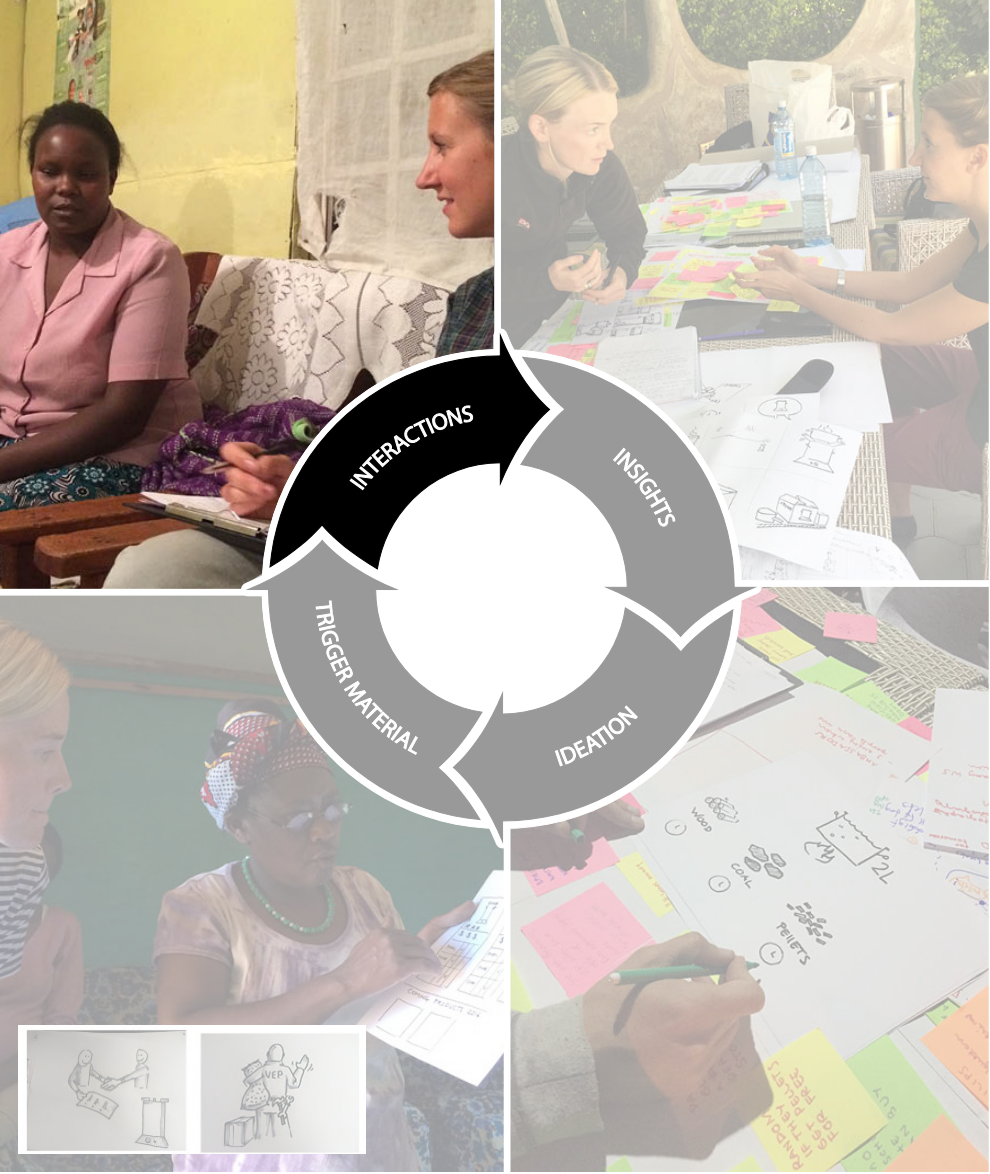
\includegraphics[width=0.7\textwidth]{Iteration.png}
    \caption{One iteration consists of Interactions, Insights, Ideation and Trigger material. The \textbf{Didactic phase} in this figure involves Insights, Ideation and Trigger material. By learning what works and not, new ideas emerge and app design is made, as well as questionnaires for evaluation. The \textbf{Technical phase} in this figure involves to code the improved app design, and evaluate how it works technically.}
    \label{fig:iteration}
\end{figure}

Each iteration ends with two check-up meetings. The first meeting is with the Experts. The next meeting is with the Partners.

The Expert group consists of Expedition Mondial and LiU Innovation. In Expert meetings, I share with them my needs. Expedition Mondial can help with the design process, and LiU Innovation can help if additional resources are needed. The meeting lasts for one hour.

The Partner group consists of most notably Iliana Björling, and preferably also Lena Tibell and Konrad Schönborn. In Partner meetings, The Analysis for the iteration is presented and discussed. Then I will propose possible decisions and discuss the alternatives. % Then I tell them about which decisions has been taken and why.
Finally, we conclude if the master thesis work is going in the right direction. These meetings should be causual and friendly, and not take a lot of time to prepare, so the next iteration can be of focus. % "Kan vara ganska vänskapligt, håll det så enkelt som möjligt så jag får tid till annat."

The time plan for the design and development phase can be seen in the section "In Uganda". The three iterations is presented below: \\

\textbf{The iterations} \\
This is how I want the process to continue:\\

	\textit{\textbf{Iteration 1}}\\
    The first iteration will have a very broad scope. The focus is on the coaches' needs, motivations, and context.  After creation of questions for questionnaire 1, I'll do interviews with coaches and other involved parties. If coaches are met in-group, open questions and dialogue will be done in group for them to be comfortable, posting anonymous answers via post-its on the wall, which leads to specific questions. These sessions will be recorded.

    %resultat: design proposal, Thoughful Interaction Design. "This is where the designer gets involved in design work, establishes a preliminary understanding of the situation, navigates through available information, and initiates all neccessary relationships with clients, users, decision makers, and so forth. Based on all this, she creates a design proposal.

    A first analysis will be done to determine needs, motivations, and expectations. Then, a summarizing meeting will be held with the expert and the partner group to determine possible ways of going forward. A first trigger/paper material will be created, for iteration 2.\\

   \textit{\textbf{Iteration 2}}\\
   This time, the iteration has a more detailed scope, with a hypothesis on what needs the app should meet and in the end, and test the trigger material created to meet those needs.

   I'll be helped with questionnaire material 2. I'll facilitate co-creating interviews with coaches, make an analysis to identify important functionality, and have a summarizing meeting with experts and partners to determine the way forward. A second trigger material will be created, one which was digital, and one which was only made on paper.\\

   \textit{\textbf{Iteration 3}}\\
   Finally, I will be supported with the third iteration, with an even more detailed scope. A co-creation workshop will be held.

   Before the workshop, the wished functionality and goals should be well formulated. Then, it can be discussed how to best design the workshop, together with Lena, Konrad, and Expedition Mondial.

   Questionnaire 3 will be created. In conjunction with the workshop the coaches can be tested, interviewed, and their interactions studied.

In the end of iteration 3, a final analysis will be done, and a final summarizing meeting with experts and partners will determine they way forward.\\


\section{Answering research questions \#1}

\textbf{\textit{How the topic of Entrepreneurship affects the work}}\\
The scope of the app is to examine the entrepreneurship the student already has. The goal is to give good feedback.

Entrepreneurship is a developing area of research. The topic and the YoungDrive's methology largely effects the work, via its ethos "Dream big, start small", "Can you sell?", and emphasis on fun. Their existing training material and the structure of the program needs to be taken in consideration.

Entrepreneurship means using a learning by doing methodology. A challenging part of the work is that YoungDrive consists of both the practical skills of the entrepreneur, theoretical material of running a business, and an entrepreneurial mindset. Therefore, both how to assess knowledge, and build habits, needs to be examined.

\textbf{\textit{How a Physical education affects the work}}\\
The physical vs. digital interplay needs to be closely examined. How does the app interplay with the physical education? For this, service design methodology will be used. \\

\textbf{\textit{How the Time Constraints and Cultural Differences affects the work}}\\

The biggest challenge with regards to time constraints and cultural differences is that it is difficult to understand the audience.\\

Action:
\begin{itemize}
    \item It led to me started planning the master thesis several months ago
    \item It led to me choosing to spend 3 months in Uganda, because the client and academy is there, and start the design process when I'm there
    \item It led me to the topic of Service Design
\end{itemize}

Positives:
\begin{itemize}
    \item I will come closer to the client and coaches by moving to Uganda, which is necessary when taking a service design approach
\end{itemize}

Negatives:
\begin{itemize}
    \item I will have limited internet outside of the work location
    \item Long distances between work place and home compared to Sweden
    \item I will still have long distances and limited access to coaches\\
\end{itemize}

These negatives needs to be overcome, by narrowing down the scope of the thesis work. \\

\textbf{\textit{How the Design Constraints affects the design process}}\\
"Simple" in this cultural setting leads to design constraints and that design methodology becomes very important.\\

\textbf{\textit{How the Technical Constraints affects the technologies used}}\\
Limitations on internet/electricity means:

\begin{itemize}
    \item Web app
    \item Localized
    \item Database
    \item Fetch/pull functionality in the app
    \item Battery preserving app needed
\end{itemize}

Also, me as a developer have limited experience of building apps, and time constraints. As such, technical compromises should be made.

Furthermore, existing tools could be used, instead of building the app from scratch. E.g. using existing tools like Knowly or Typeform\footnote{examples include https://showroom.typeform.com/to/ggBJPd and https://showroom.typeform.com/report/njdbt5/dIzi} during the first iterations for understanding users, and during development e.g. the Typeform API (http://typeform.io/). The Typeform API allows developers to create surveys from within their own applications or systems. \\


\subsection{Considerations, answering research question \#2}

\subsubsection{Consequences}

To be able to answer research question \#2, evaluation needs to be done. \textbf{\textit{How the Evaluation affects the development process: }} If no evaluation, there would be no need to write code, instead of working with a hi-fi prototype by using existing design tools. Now, we want to use a data-driven approach to measure, and therefore an app needs to be developed.\\

\subsubsection{How to measure}

Answering research question \#2 is a matter of choosing how to measure effectiveness. After choosing what should be evaluated, there needs to be a careful balance between what should be understood via interviews with the target group, and data collection via the app. There are three main aspects that are interesting:

These ways of measuring the questions are subject to change.

%Effectiveness measurements.

\begin{itemize}
    \item 
    \textbf{How do users interact with the app?} (Usability) Give the users a mandatory task (e.g. use the app once a week), and see if they use it more on a voluntary basis, in order to determine if they use the app 
    \textit{(Measure)} and determine why \textit{(Interview and Measurement)}. "Have you during the latest week felt that you've needed any support? Have you then used the app? Did the app help? Or have you searched for support elsewhere?" 
\item \textbf{What usability aspects are associated with using the app?} (Usability) Do they like it? Ask: Are they stimulated? If not, why? What didn't they like? \textit{(Interview)} When can they use the app, and when are they not able to?
    
    \item \textbf{What learning outcomes are associated with using the app for the coaches?}  (Learning of Entrepreneurial Knowledge))
    How good are they at answering the questions? 1. 
    \textit{(Measure)} What percentage of the answers were correct/inorrect?  2. \textit{(Interview)} Were the answers were correct/incorrect because of lack of knowledge or wrong formulated?
    
    Ask the teacher/country manager/project leader if they got valuable information. Ask: did it help them become a better teacher? Were the results trustworthy? \textit{(Interview)}
    
    Do they want to improve their knowledge via the app? This can be measured via how many times they repeat a test, what material they are studying for (e.g. measuring active time spent reading each section).
\end{itemize}
